\documentclass{beamer}

\usepackage[utf8]{inputenc}
\usepackage[T1]{fontenc}
\usepackage[ngerman]{babel}
\usepackage{amssymb}
\usepackage{graphicx} % Bilder
\usepackage{wrapfig} % Umflussbilder
\usepackage{multicol} % Multiple columns
\usepackage{minted} % Haskell source code
\usepackage{framed} % Frames around source code
\usepackage[framemethod=tikz]{mdframed} % Frames
\usepackage{verbatim} % \begin{comment}...\end{comment}
\usepackage{etoolbox} % manipulate minted
\AtBeginEnvironment{minted}{\fontsize{10}{10}\selectfont}
\AfterEndEnvironment{minted}{}

\mdfdefinestyle{fancy}{
  roundcorner=5pt,
  linewidth=4pt,
  linecolor=red!80,
  backgroundcolor=red!20
}
\newmdenv[style=fancy]{important}

% redifine \em for \emph to use bold instead of italics
\makeatletter
\DeclareRobustCommand{\em}{%
  \@nomath\em \if b\expandafter\@car\f@series\@nil
  \normalfont \else \bfseries \fi}
\makeatother

% Stuff for Beamer
\beamertemplatenavigationsymbolsempty
\usetheme{Warsaw}

\title{Fortgeschrittene Funktionale Programmierung in Haskell}

\begin{document}
  
%----------------------------------------------------------------------------------------  

  \begin{frame}
  \begin{center}
    \huge\textbf{Fortgeschrittene Funktionale Programmierung in Haskell}\\ \bigskip
    \LARGE Universität Bielefeld, Sommersemester 2015\\ \bigskip
    \large Jonas Betzendahl \& Stefan Dresselhaus
    \end{center}
  \end{frame}
  
%----------------------------------------------------------------------------------------

\begin{frame}
\frametitle{Orga-Krams}

Heute ist die letzte Vorlesung, die Deadline für die Projekte ist am Freitag, den 18.09.2015. Ab sofort nehmen wir Abgaben für die Projekte entgegen.

Für eine Abgabe schreibt bitte eine Mail an beide Tutoren (\texttt{sdressel@techfak...} und \texttt{jbetzend@techfak...}) mit entweder dem kompletten Quellcode oder einem Link auf einen Tag auf \texttt{github.com}.\pause\bigskip

Besonderer Dank geht an Alexander Sczyrba und Mario Botsch, dafür dass es uns möglich gemacht wurde, diese Vorlesung überhaupt zu halten, an alle, die uns bei der Durchführung geholfen haben und natürlich an alle, die mitgemacht haben. 
\end{frame}

%----------------------------------------------------------------------------------------
\section*{Alligator Eggs}
%----------------------------------------------------------------------------------------

\begin{frame}

\begin{center}
\Large \textbf{Alligator Eggs} \tiny \bigskip

Idee \& Bilder: Bret Victor\\
\texttt{http://worrydream.com/AlligatorEggs/}
\end{center}

\end{frame}

%----------------------------------------------------------------------------------------
\subsection*{Konzept}

\begin{frame}
Wir betrachten heute ein Spiel, das gleichzeitig bunt und putzig ist und uns erlaubt,
etwas interessantes zu lernen! Es gibt\dots \pause\smallskip

\begin{itemize}
\item \textbf{Hungrige Alligatoren}\\
      
\includegraphics[scale=0.2]{pieces_1.png}\\
      Hungrige Alligatoren sind hungrig! Sie fressen alles, was ihnen vor's Maul kommt.
      Sie bewachen aber außerdem ihre Familien.
      \pause
\item \textbf{Alte Alligatoren}\\
      
\includegraphics[scale=0.2]{pieces_2.png}\\
      Diese Alligatoren haben genug gegessen und bewachen nur noch ihre Familien.
      \pause
\item \textbf{Alligatoreier}\\
      
\includegraphics[scale=0.2]{pieces_3.png}\\
      Aus Eiern schlüpfen demnächst neue Alligatorfamilien.
\end{itemize}

\end{frame}

%----------------------------------------------------------------------------------------

\begin{frame}
\frametitle{Familien}

Alligatoren kommen in Familien daher. Hier ist eine:

\begin{multicols}{2}

\begin{center}

\includegraphics[scale=0.6]{families_1.png} 
\end{center}

\columnbreak
\pause

Hier ist noch nicht viel zu sehen, was wirklich interessiert.\smallskip\smallskip

Nur ein grüner Alligator, der sein grünes Ei bewacht.\\Ist er nicht süß?

\end{multicols}

\end{frame}

%----------------------------------------------------------------------------------------

\begin{frame}
\frametitle{Familien}

Hier ist eine weitere Familie, dieses Mal mit mehr Mitgliedern.\pause

\begin{multicols}{2}

\begin{center}
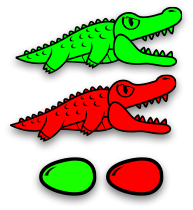
\includegraphics[scale=0.6]{families_2.png} 
\end{center}

\columnbreak

Ein grüner und ein roter Alligator bewachen ein grünes und ein rotes Ei.\bigskip

Oder anders formuliert:

Ein grüner Alligator bewacht einen roten Alligator und der rote Alligator bewacht die zwei Eier.

\end{multicols}

\end{frame}

%----------------------------------------------------------------------------------------

\begin{frame}
\frametitle{Familien}

Dieses Mal haben wir eine richtige Großfamilie:\pause

\begin{multicols}{2}

\begin{center}
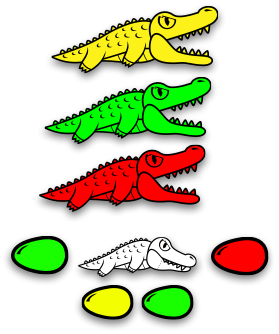
\includegraphics[scale=0.5]{families_3.png} 
\end{center}

\columnbreak
\pause

Hier haben wir drei hungrige Alligatoren, die Wache halten. Einen gelben, einen grünen und einen roten.\pause\bigskip

Sie bewachen drei Dinge: Ein grünes Ei, einen alten Alligator und ein rotes Ei.\pause\bigskip

Der alte Alligator hingegen bewacht ein gelbes und ein grünes Ei. 

\end{multicols}

\end{frame}

%----------------------------------------------------------------------------------------
\subsection*{Beispiel}

\begin{frame}
\frametitle{Fressen und gefressen werden}

\begin{center}
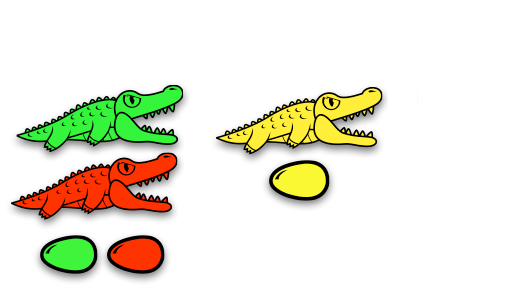
\includegraphics[scale=0.45]{eating_1.png} 
\end{center}
\bigskip

Hier wird es etwas ungemütlicher. Wir sehen hier zwei Familien nebeneinander.
\end{frame}

%----------------------------------------------------------------------------------------

\begin{frame}
\frametitle{Fressen und gefressen werden}

\begin{center}
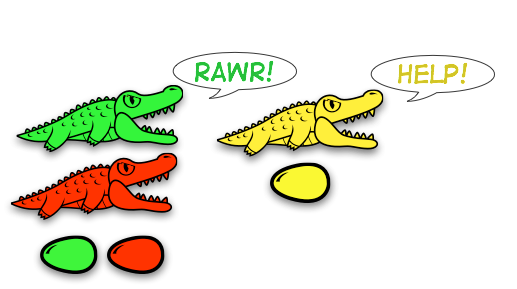
\includegraphics[scale=0.45]{eating_2.png} 
\end{center}
\bigskip

Hier wird es etwas ungemütlicher. Wir sehen hier zwei Familien nebeneinander. Der grüne Alligator ist \emph{sehr} hungrig\dots
\end{frame}

%----------------------------------------------------------------------------------------

\begin{frame}
\frametitle{Fressen und gefressen werden}

\begin{center}
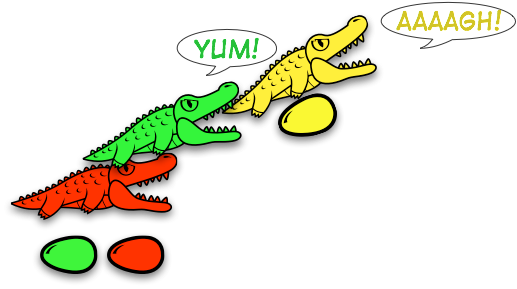
\includegraphics[scale=0.45]{eating_3.png} 
\end{center}
\bigskip

Hier wird es etwas ungemütlicher. Wir sehen hier zwei Familien nebeneinander. Der grüne Alligator ist \emph{sehr} hungrig\dots
\end{frame}

%----------------------------------------------------------------------------------------

\begin{frame}
\begin{multicols}{2}
\frametitle{Fressen und gefressen werden}

\begin{center}
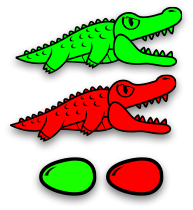
\includegraphics[scale=0.45]{families_2.png} 
\end{center}
\columnbreak

Der grüne Alligator hat die komplette gelbe Familie gefressen.

\end{multicols}
\end{frame}

%----------------------------------------------------------------------------------------

\begin{frame}
\begin{multicols}{2}
\frametitle{Fressen und gefressen werden}

\begin{center}
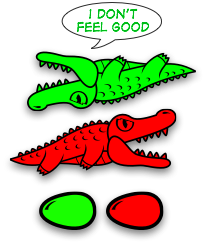
\includegraphics[scale=0.45]{eating_4.png} 
\end{center}
\columnbreak

Der grüne Alligator hat die komplette gelbe Familie gefressen. Das war allerdings zu viel für seinen Magen. Er hat sich überfressen und stirbt.

\end{multicols}
\end{frame}

%----------------------------------------------------------------------------------------

\begin{frame}
\begin{multicols}{2}
\frametitle{Fressen und gefressen werden}

\begin{center}
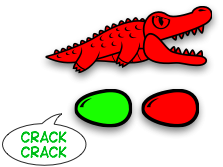
\includegraphics[scale=0.45]{eating_5.png} 
\end{center}
\columnbreak

Was übrig bleibt ist der rote Alligator. Jetzt wo sein grüner Freund gestorben ist, fängt jedoch das grüne Ei an, zu schlüpfen.

\end{multicols}
\end{frame}

%----------------------------------------------------------------------------------------

\begin{frame}
\begin{multicols}{2}
\frametitle{Fressen und gefressen werden}

\begin{center}
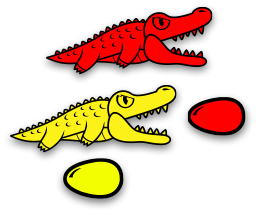
\includegraphics[scale=0.45]{eating_6.png} 
\end{center}
\columnbreak

Was übrig bleibt ist der rote Alligator. Jetzt wo sein grüner Freund gestorben ist, fängt jedoch das grüne Ei an, zu schlüpfen.

Es schlüpft \emph{exakt}, was der grüne Alligator gerade gegessen hat. Das Wunder des Lebens!

\end{multicols}
\end{frame}

%----------------------------------------------------------------------------------------

\begin{frame}
\begin{multicols}{2}
\frametitle{Fressen und gefressen werden}

\begin{center}
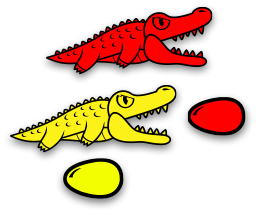
\includegraphics[scale=0.45]{eating_6.png} 
\end{center}
\columnbreak

Was übrig bleibt ist der rote Alligator. Jetzt wo sein grüner Freund gestorben ist, fängt jedoch das grüne Ei an, zu schlüpfen.

Es schlüpft \emph{exakt}, was der grüne Alligator gerade gegessen hat. Das Wunder des Lebens!

\end{multicols}
\end{frame}

%----------------------------------------------------------------------------------------

\begin{frame}
\begin{multicols}{2}
\frametitle{Fressen und gefressen werden}

\begin{center}
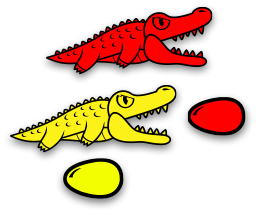
\includegraphics[scale=0.45]{eating_6.png} 
\end{center}
\columnbreak

Jetzt ist also eine neue gelbe Familie geschlüpft. 

\end{multicols}
\end{frame}


%----------------------------------------------------------------------------------------

\begin{frame}
\begin{multicols}{2}
\frametitle{Fressen und gefressen werden}

\begin{center}
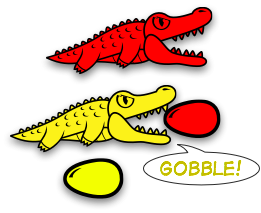
\includegraphics[scale=0.45]{eating_7.png} 
\end{center}
\columnbreak

Jetzt ist also eine neue gelbe Familie geschlüpft. Allerdings ist dieser gelbe Alligator auch ziemlich hungrig\dots

\end{multicols}
\end{frame}

%----------------------------------------------------------------------------------------

\begin{frame}
\begin{multicols}{2}
\frametitle{Fressen und gefressen werden}

\begin{center}
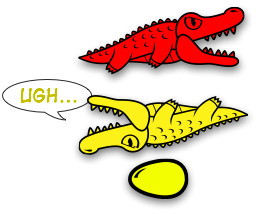
\includegraphics[scale=0.45]{eating_8.png} 
\end{center}
\columnbreak

Jetzt ist also eine neue gelbe Familie geschlüpft. Allerdings ist dieser gelbe Alligator auch ziemlich hungrig\dots

Nachdem er das rote Ei gefressen hat, ist allerdings auch sein Magen schon zu voll und ihn ereilt das gleiche Schicksal wie den grünen Alligator.

\end{multicols}
\end{frame}

%----------------------------------------------------------------------------------------

\begin{frame}
\begin{multicols}{2}
\frametitle{Fressen und gefressen werden}

\begin{center}
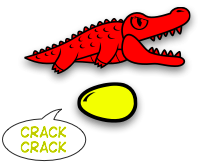
\includegraphics[scale=0.45]{eating_9.png} 
\end{center}
\columnbreak

Jetzt ist also eine neue gelbe Familie geschlüpft. Allerdings ist dieser gelbe Alligator auch ziemlich hungrig\dots

Nachdem er das rote Ei gefressen hat, ist allerdings auch sein Magen schon zu voll und ihn ereilt das gleiche Schicksal wie den grünen Alligator. Und auch aus diesem Ei schlüpft, was gerade gegessen wurde.

\end{multicols}
\end{frame}

%----------------------------------------------------------------------------------------

\begin{frame}
\begin{multicols}{2}
\frametitle{Fressen und gefressen werden}

\begin{center}

\includegraphics[scale=0.45]{eating_10.png} 
\end{center}
\columnbreak

Jetzt ist also eine neue gelbe Familie geschlüpft. Allerdings ist dieser gelbe Alligator auch ziemlich hungrig\dots

Nachdem er das rote Ei gefressen hat, ist allerdings auch sein Magen schon zu voll und ihn ereilt das gleiche Schicksal wie den grünen Alligator. Und auch aus diesem Ei schlüpft, was gerade gegessen wurde.

Hier endet das Drama, da es nichts mehr zum Fressen gibt.

\end{multicols}
\end{frame}

%----------------------------------------------------------------------------------------
\subsection*{Formale Regeln}

\begin{frame}
\frametitle{Die Essensregel}

Wir können jetzt eine erste \glqq formale\grqq\ Regel für dieses System aufstellen:\bigskip\pause

Wenn wir Alligatorfamilien nebeneinander haben, \dots\bigskip

\begin{center}
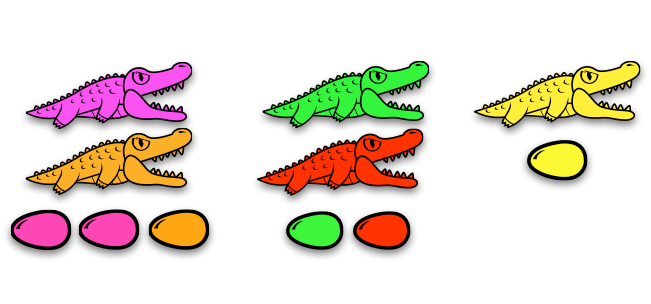
\includegraphics[scale=0.35]{eatingrule_1.png} 
\end{center}

\end{frame}

%----------------------------------------------------------------------------------------

\begin{frame}
\frametitle{Die Essensregel}

Wir können jetzt eine erste \glqq formale\grqq\ Regel für dieses System aufstellen:\bigskip

Wenn wir Alligatorfamilien nebeneinander haben, frisst der Alligator links oben die Familie rechts neben ihm.\bigskip

\begin{center}
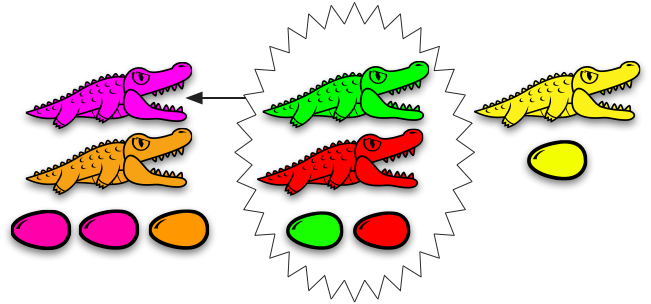
\includegraphics[scale=0.35]{eatingrule_2.png} 
\end{center}

\end{frame}

%----------------------------------------------------------------------------------------

\begin{frame}
\frametitle{Die Essensregel}

Wenn wir Alligatorfamilien nebeneinander haben, frisst der Alligator links oben die Familie rechts neben ihm. Dieser Alligator stirbt. Bewacht seine Familie jedoch Eier seiner Farbe, schlüpft aus \emph{jedem} dieser Eier, was er gerade noch verspeist hat.

\begin{center}
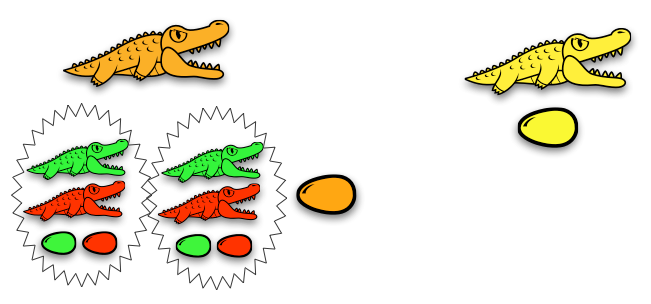
\includegraphics[scale=0.4]{eatingrule_3.png} 
\end{center}

\end{frame}

%----------------------------------------------------------------------------------------

\begin{frame}
\frametitle{Die Farbenregel}

\begin{center}
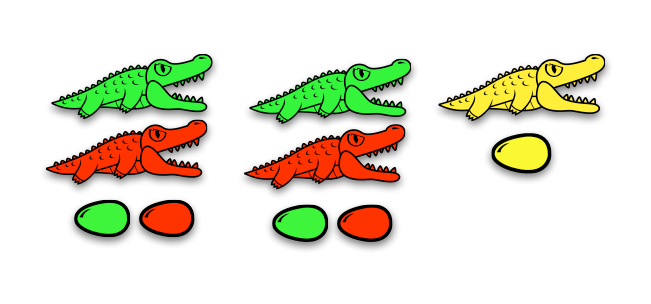
\includegraphics[scale=0.35]{eatingrule_4.png} 
\end{center}

Setzen wir das Beispiel fort, frisst Orange Gelb und wir verbleiben mit dieser Konstellation.
Jetzt gibt es allerdings ein Problem.

\end{frame}

%----------------------------------------------------------------------------------------

\begin{frame}
\frametitle{Die Farbenregel}

\begin{center}
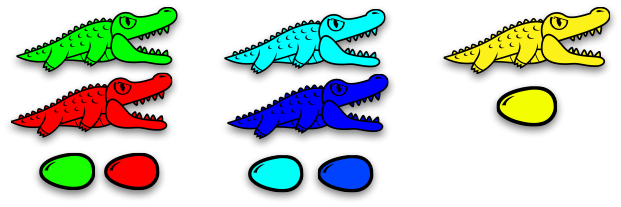
\includegraphics[scale=0.35]{colorrule_1.png} 
\end{center}

Setzen wir das Beispiel fort, frisst Orange Gelb und wir verbleiben mit dieser Konstellation.
Jetzt gibt es allerdings ein Problem.

Bevor ein Alligator eine Familie essen kann, in der eine Farbe vorkommt, die auch eins seiner Familienmitglieder hat, müssen die Farben geändert werden.

\end{frame}

%----------------------------------------------------------------------------------------

\begin{frame}
\frametitle{Die Farbenregel}

\begin{center}
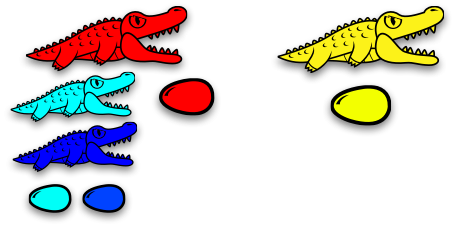
\includegraphics[scale=0.35]{colorrule_2.png} 
\end{center}

Setzen wir das Beispiel fort, frisst Orange Gelb und wir verbleiben mit dieser Konstellation.
Jetzt gibt es allerdings ein Problem.

Bevor ein Alligator eine Familie essen kann, in der eine Farbe vorkommt, die auch eins seiner Familienmitglieder hat, müssen die Farben geändert werden.

Dann können wir essen\dots

\end{frame}

%----------------------------------------------------------------------------------------

\begin{frame}
\frametitle{Die Farbenregel}

\begin{center}
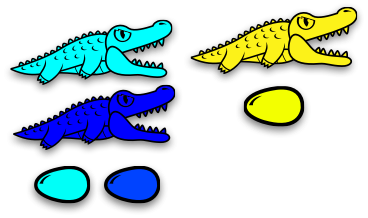
\includegraphics[scale=0.35]{colorrule_3.png} 
\end{center}

Setzen wir das Beispiel fort, frisst Orange Gelb und wir verbleiben mit dieser Konstellation.
Jetzt gibt es allerdings ein Problem.

Bevor ein Alligator eine Familie essen kann, in der eine Farbe vorkommt, die auch eins seiner Familienmitglieder hat, müssen die Farben geändert werden.

Dann können wir essen und essen\dots

\end{frame}

%----------------------------------------------------------------------------------------

\begin{frame}
\frametitle{Die Farbenregel}

\begin{center}
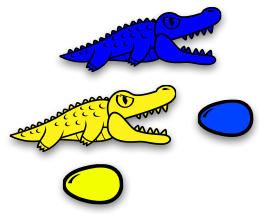
\includegraphics[scale=0.35]{colorrule_4.png} 
\end{center}

Setzen wir das Beispiel fort, frisst Orange Gelb und wir verbleiben mit dieser Konstellation.
Jetzt gibt es allerdings ein Problem.

Bevor ein Alligator eine Familie essen kann, in der eine Farbe vorkommt, die auch eins seiner Familienmitglieder hat, müssen die Farben geändert werden.

Dann können wir essen und essen und essen\dots

\end{frame}

%----------------------------------------------------------------------------------------

\begin{frame}
\frametitle{Die Farbenregel}

\begin{center}
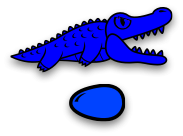
\includegraphics[scale=0.45]{colorrule_5.png} 
\end{center}

Setzen wir das Beispiel fort, frisst Orange Gelb und wir verbleiben mit dieser Konstellation.
Jetzt gibt es allerdings ein Problem.

Bevor ein Alligator eine Familie essen kann, in der eine Farbe vorkommt, die auch eins seiner Familienmitglieder hat, müssen die Farben geändert werden.

Dann können wir essen und essen und essen, bis alles weg ist.

\end{frame}

%----------------------------------------------------------------------------------------

\begin{frame}
\frametitle{Die Altersschwächeregel}

\begin{center}
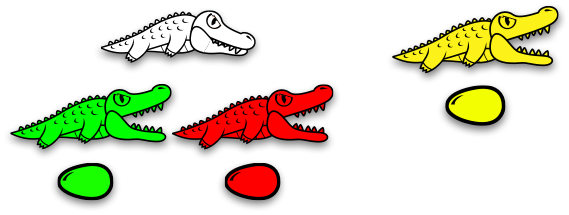
\includegraphics[scale=0.35]{old_1.png} 
\end{center}

Es gibt noch eine weitere Regel, die wir beachten müssen. Sie betrifft alte Alligatoren, die nicht mehr hungrig sind und nur noch ihre Familie bewachen (wie hier oben links). Unter welchen Bedingungen sterben diese?

\end{frame}

%----------------------------------------------------------------------------------------

\begin{frame}
\frametitle{Die Altersschwächeregel}

\begin{center}

\includegraphics[scale=0.35]{old_2.png} 
\end{center}

Die Antwort ist, dass sie sterben, wenn sie nur noch eine Familie beschützen.\bigskip

Hier frisst der grüne Alligator die rote Familie und stirbt. Danach schlüpft eine neue rote Familie aus dem grünen Ei. Der alte Alligator bewacht jetzt nur noch eine Familie, die auch auf sich allein aufpassen kann. Er wird nicht mehr gebraucht, also stirbt er.

\end{frame}

%----------------------------------------------------------------------------------------

\begin{frame}
\frametitle{Die Altersschwächeregel}

\begin{center}
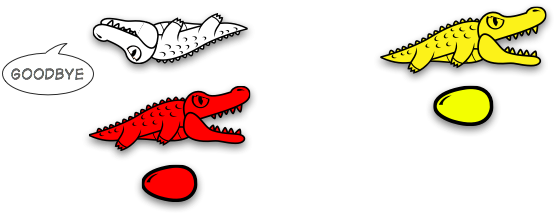
\includegraphics[scale=0.35]{old_3.png} 
\end{center}

Die Antwort ist, dass sie sterben, wenn sie nur noch eine Familie beschützen.\bigskip

Hier frisst der grüne Alligator die rote Familie und stirbt. Danach schlüpft eine neue rote Familie aus dem grünen Ei. Der alte Alligator bewacht jetzt nur noch eine Familie, die auch auf sich allein aufpassen kann. Er wird nicht mehr gebraucht, also stirbt er.

\end{frame}

%----------------------------------------------------------------------------------------

\begin{frame}
\frametitle{Die Altersschwächeregel}

\begin{center}

\includegraphics[scale=0.35]{old_4.png} 
\end{center}

Die Antwort ist, dass sie sterben, wenn sie nur noch eine Familie beschützen.\bigskip

Hier frisst der grüne Alligator die rote Familie und stirbt. Danach schlüpft eine neue rote Familie aus dem grünen Ei. Der alte Alligator bewacht jetzt nur noch eine Familie, die auch auf sich allein aufpassen kann. Er wird nicht mehr gebraucht, also stirbt er.
Danach rückt der rote hungrige Alligator nach und frisst.

\end{frame}

%----------------------------------------------------------------------------------------

\begin{frame}
\frametitle{Die Altersschwächeregel}

\begin{center}

\includegraphics[scale=0.35]{old_5.png} 
\end{center}

Die Antwort ist, dass sie sterben, wenn sie nur noch eine Familie beschützen.\bigskip

Hier frisst der grüne Alligator die rote Familie und stirbt. Danach schlüpft eine neue rote Familie aus dem grünen Ei. Der alte Alligator bewacht jetzt nur noch eine Familie, die auch auf sich allein aufpassen kann. Er wird nicht mehr gebraucht, also stirbt er.
Danach rückt der rote hungrige Alligator nach und frisst. Und so weiter und so fort, bis nichts mehr da ist.

\end{frame}

%----------------------------------------------------------------------------------------

\begin{frame}
\frametitle{Gameplay}

Das Ziel des Spiels ist nun, eine Familie auszuknobeln, die, wenn sie $X$ gefüttert bekommt, $Y$ produziert. Wir betrachten dabei zwei Familien unterschiedlicher Farben als \glqq äquivalent\grqq , wenn sie das gleiche Muster haben. Ein Beispiel:\pause

\begin{multicols}{2}

Hier sind zwei Familien, die wir \glqq \texttt{True}\grqq und \glqq \texttt{False}\grqq\ nennen:

\begin{center}
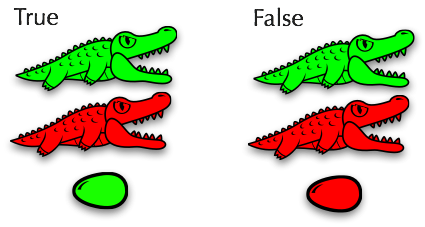
\includegraphics[scale=0.25]{gameplay_1.png} 
\end{center}

\columnbreak
\pause

Und hier ist die Familie \glqq \texttt{Not}\grqq :

\begin{center}
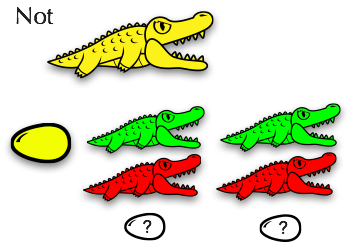
\includegraphics[scale=0.3]{gameplay_2.png} 
\end{center}

\end{multicols}

Frage: Welche Farbe müssten die Eier der Familie \texttt{Not} haben?

\end{frame}

%----------------------------------------------------------------------------------------

\begin{frame}

Eine kleine Aufgabe, die eigentlich auf einem Übungszettel hätte landen sollen:\pause\bigskip

Implementieren Sie eine kleine Alligator-DSL (Domain Specific Language) in \texttt{Haskell}, die einen gegebenen \glqq Alligator-Ausdruck\grqq\ (grafisch?) auswertet.\bigskip

Implementieren Sie außerdem die Konnektive \texttt{AND}, \texttt{OR}, \texttt{NAND} und \texttt{XOR} als Alligator-Ausdrücke. 

\end{frame}

%----------------------------------------------------------------------------------------
\section*{Lambda-Kalkül}
%----------------------------------------------------------------------------------------

\begin{frame}

\begin{center}
\Large $\lambda$-\textbf{Kalkül} \& $\lambda$-\textbf{Würfel} \normalsize
\end{center}

\end{frame}

\subsection*{Lambda-Kalkül}

\begin{frame}
Was ist ein Lambdakalkül (engl. $\lambda$-calculus) und warum interessiert mich das?
\pause\bigskip

Das Lambdakalkül wurde in den 1930ern von Alonzo Church entworfen und formalisiert das Konzept \glqq Berechnung\grqq. Man könnte sagen, es ist die kleinste universelle Programmiersprache. 

Heute noch spielt sie große Rollen in Programmiersprachentheorie. \texttt{Haskell} z.B. basiert auf dem Lambdakalkül.\smallskip\smallskip

Empfehlung: Philipp Wadler (Prof. in Edinburgh) stand-up comedy zu computability theory:
\url{https://www.youtube.com/watch?v=GnpcMCW0RUA}

\pause\bigskip
\dots und lustigerweise ist all das äquivalent zu unseren Alligator-Ausdrücken!
\end{frame}

%----------------------------------------------------------------------------------------

\begin{frame}
\frametitle{Lambda-Calculus}

Das Lambdakalkül setzt sich aus zwei Dingen zusammen: gültige \emph{Terme} und \emph{Umformungsregeln}
zwischen Termen.\smallskip\smallskip\smallskip

Ein gültiger Term ist eins von drei Dingen:
\begin{itemize}
\pause\item Eine Variable, (z.B.: $a,b,c,\dots$)
\pause\item Eine Lambda-Abstraktion (z.B.: $\lambda x . xx$)
\pause\item Eine Anwendung eines Terms auf einen anderen
            \\ (z.B.: $(\lambda x . xx)(palim)$)
\end{itemize}
\end{frame}

%----------------------------------------------------------------------------------------

\begin{frame}
\frametitle{$\alpha$-Konversion}

Die erste Konversionsregel wird $\alpha$-Konversion, oder Umbenennung genannt:

$$ \lambda V . E \equiv \lambda W.E [V \leftarrow W]$$
\pause

Diese Regel besagt quasi, dass Variablennamen irrelephant sind. $(\lambda x . xx)$ und $(\lambda y . yy)$ sind diesselbe Funktion. Die Details sind allerdings etwas komplizierter, wir werden hier nicht näher drauf eingehen.
\pause

Können zwei Terme ineinander umgewandelt werden, nennt man sie $\alpha$-äquivalent. Meistens werden $\alpha$-äquivalente Terme als identisch angesehen.
\end{frame}

%----------------------------------------------------------------------------------------

\begin{frame}
\frametitle{$\beta$-Reduktion}

Die zweite Konversionsregel, genannt $\beta$-Reduktion, bildet das Konzept von Funktionsanwendung ab:

$$ (\lambda V . E) E' \equiv E [V \leftarrow E'] $$
\pause

Hier wird einfach das Argument an die Stelle der Variablen eingesetzt. Eine Bedingung ist allerdings,
dass alle freien Variablen frei bleiben müssen.\pause

Terme, auf die diese Regel angewandt werden kann, heißen $\beta$-reduzibel. Allerdings haben nicht alle Terme auch eine $\beta$-Normalform ($(\lambda x.xx)(\lambda x.xx)$ z.B. ist reduzibel, ergibt sich aber selbst).
\end{frame}

%----------------------------------------------------------------------------------------

\begin{frame}
\frametitle{$\eta$-Konversion}

Die dritte Konversionsregel, genannt $\eta$-Konversion, ist lediglich optional:

$$ \lambda x . f x \equiv f$$
\pause

Bedingung ist, dass $x$ keine freie Variable von $f$ ist. Diese Regel kann hinzugefügt werden, wenn man \emph{Extensionalität} abbilden möchte. Das bedeutet, dass zwei Funktionen gleich sind, wenn sie für alle Eingaben das gleiche Ergebnis liefern.\pause\bigskip

\textbf{Beispiel:} \texttt{quicksort} und \texttt{heapsort} sind \emph{extensional} gleich
\\($\forall x . $ \texttt{mergesort}$(x) = $\texttt{ heapsort}$(x) $), \emph{intensional} allerdings nicht.
\end{frame}

%----------------------------------------------------------------------------------------

\begin{frame}
\frametitle{Lambda calculus-Alligator-Isomorphism}

Wie vorhin versprochen gibt es eine genaue Übersetzung von unseren Alligatoren zum
Lambda-Kalkül und umgekehrt:\pause\bigskip

\begin{center}
\begin{tabular}{c|c}
\textbf{Alligatoren} & \textbf{Lambda-Kalkül}\\
\hline
\\
Hungriger Alligator & Lambda-Abstraktion\\
Eier & Variablen\\
Alter Alligator & Klammern\\
&\\
Essensregel & $\beta$-Reduktion\\
Farbenregel & $\alpha$-Konversion\\
Altersregel & Klammern löschen\\ 

\end{tabular}
\end{center}

\end{frame}

%----------------------------------------------------------------------------------------
\subsection*{Lambda-Würfel}

\begin{frame}

Das Lambdakalkül mit Typen (eine Einschränkung des untypisierten Kalküls) ist allerdings nur der Anfang. Im so genannten \glqq Lambda-Würfel\grqq\ ist es der Ursprung ($\lambda\to$).\pause

\begin{multicols}{2}
\begin{center}
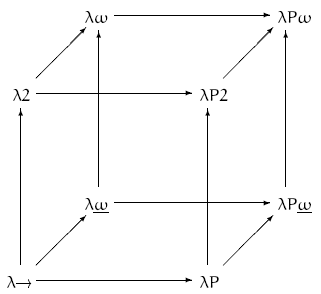
\includegraphics[scale=0.4]{Lambda_cube.png} 
\end{center}
\columnbreak

Im Würfel gibt es drei Richtungen der Abstraktion:\smallskip\smallskip

\begin{itemize}
\pause\item \textit{Terms depending on types}
            \\ Auch \glqq Polymorphismus\grqq\
\pause\item \textit{Types depending on types}
            \\ Auch \glqq Type Operators\grqq\
\pause\item \textit{Types depending on terms}
            \\ Auch \glqq Dependent Types\grqq\
\end{itemize}

\end{multicols}
\pause

Das obere Ende des Würfels, $\lambda\Pi\omega$, ist auch als \glqq calculus of constructions\grqq\ bekannt (entwickelt von Thierry Coquand) und dient als Basis für den Beweisassistenten \texttt{Coq}.

\end{frame}

%----------------------------------------------------------------------------------------
\section*{Kategorientheorie 101}
%----------------------------------------------------------------------------------------

\begin{frame}

\begin{center}
Back to the roots:\\
\Large \textbf{Monads \& Categories}
\end{center}

\end{frame}

%----------------------------------------------------------------------------------------

\begin{frame}
Zum Abschluss wollen wir noch ein besonders bekanntes Meme der Haskell-Community genauer
unter die Lupe nehmen. Den Satz:

\begin{center}
\textit{\glqq Monaden sind Monoide in der Kategorie der Endofunktoren.\grqq}
\end{center}
\pause

\dots dafür werden wir allerdings einen kleinen Abstecher in die Mathematik benötigen.
\end{frame}

%----------------------------------------------------------------------------------------
\subsection*{Monads}

\begin{frame}[fragile]

\underline{Eine kurze Erinnerung:}\bigskip

\texttt{Monad} ist eine Typklasse in \texttt{Haskell}, die die Implementation von \texttt{return} und \texttt{>>=} (Bind) voraussetzt. Insbesondere ist jeder Typ in \texttt{Monad} ebenfalls in \texttt{Applicative} und \texttt{Functor}.\bigskip

\begin{minted}{haskell}
class Applicative m => Monad m where
    return :: a -> m a
    (>>=)  :: m a -> (a -> m b) -> m b
\end{minted}
\pause

Besonders beliebt: \texttt{Identity, [], IO, Maybe}\dots
\end{frame}

%----------------------------------------------------------------------------------------

\begin{frame}[fragile]

Statt \texttt{return} und \texttt{(>>=)} kann man auch andere Funktionen verwenden.
In der Kategorientheorie werden häufig $\eta : I \to M$ (unit) und $\mu : M \times M \to M$ (join) verwendet.
\pause

\begin{multicols}{2}

\begin{center}
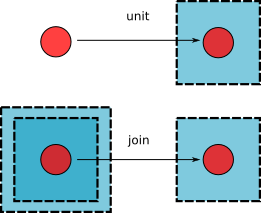
\includegraphics[scale=0.4]{Unit-join.png} 
\end{center}

\columnbreak
\pause

\begin{minted}{haskell}
unit :: Monad m -> a -> m a
unit = return

join :: Monad m => m (m a)
                -> m a
join x = x >>= id

(>>=) :: Monad m => m a
                 -> (a -> m b)
                 -> m b
x >>= f = join (fmap f x)
\end{minted}

\end{multicols}


\end{frame}

%----------------------------------------------------------------------------------------
\subsection*{Monoids}

\begin{frame}
\underline{\emph{Definition (Algebra):}}\\ Sei $M$ eine Menge und $\circ$ eine (abgeschl.) binäre Relation auf $M$ (d.h. $\circ : M \times M \to M$). Dann heißt $(M, \circ)$ \emph{Monoid}, wenn $\circ$ die folgenden zwei Axiome beachtet:

\begin{itemize}
\pause \item \texttt{(ass)} $\forall a,b,c \in M:\; (a \circ b) \circ c = a \circ (b \circ c)$
\pause \item \texttt{(ide)} $\exists e \in M$ sodass $\forall a \in m:\; e \circ a = a \circ e = a$
\end{itemize}
\pause\bigskip

Beliebte Monoide:
\begin{itemize}
\pause \item $(\mathbb{N}, +), (\mathbb{N}, \cdot), (\{\bot, \top\}$, \texttt{AND}$), (\{\bot, \top\}$, \texttt{OR}$)$\dots
\pause \item Gegeben eine Menge $A$, $\mathcal{P}(A)$ entweder mit $\cap$ oder $\cup$
\pause \item Jede Menge mit nur einem Element formt einen trivialen Monoid mit der trivialen Relation.
\end{itemize}

\end{frame}

%----------------------------------------------------------------------------------------
\subsection*{Categories}

\begin{frame}
\frametitle{Kategorientheorie}

Worum geht es bei Kategorientheorie?
\pause\bigskip

Kategorientheorie kann als die \glqq Mathematik der Mathematik\grqq\ betrachtet werden. Es geht um eine
Abstraktion vieler Konzepte aus unterschiedlichen Zweigen der Mathematik und die Aufdeckung fundamentaler
Ähnlichkeiten zwischen ihnen.
\pause\bigskip

\textit{\glqq Category theory has been labelled as 'generalised abstract nonsense' by both its critics and 
its proponents!\grqq}
\end{frame}

%----------------------------------------------------------------------------------------

\begin{frame}
\frametitle{Kategorientheorie}

Eine Kategorie, oft genannt $\mathcal{C}$, besteht aus:
\begin{itemize}
\pause\item Einer Klasse (engl. \glqq collection\grqq , keine Menge!) aus \emph{Objekten}, genannt $Obj(\mathcal{C})$.
\pause\item Einer Klasse von \emph{Pfeilen} (oder auch \emph{Morphismen}) zwischen Objekten, genannt $Hom(\mathcal{C})$. Ein Morphismus in $\mathcal{C}$ von Element $X$ zu Element $Y$ wird oft als $Hom_\mathcal{C}(X,Y)$ notiert.
\pause\item Einer assoziativen Verknüpfungsrelation für Morphismen:
$$Hom_\mathcal{C}(Y,Z) \times Hom_\mathcal{C}(X,Y) \to Hom_\mathcal{C}(X,Z)$$
$$(g,f) \mapsto g \circ f$$
\pause\item Einem Identitätsmorphismus für jedes Objekt $X$, notiert als $id_X$, der als neutrales Element für die Verknüpfung von Morphismen mit Domäne oder Codomäne $X$ fungiert.
\end{itemize}
\end{frame}

%----------------------------------------------------------------------------------------

\begin{frame}
\frametitle{Funktoren}
Und was ist mit Funktoren?\pause\bigskip

Seien $\mathcal{C}$ und $\mathcal{D}$ Kategorien. Ein \emph{Funktor} $F$ ist eine Abbildung
von $\mathcal{C}$ nach $\mathcal{D}$, die folgende Bedingungen einhält:

\begin{itemize}
\pause \item $F$ bildet jedes $X \in Obj(\mathcal{C})$ auf ein $F(X) \in Obj(\mathcal{D})$ ab.
\pause \item $F$ bildet jedes $f \in Hom(\mathcal{C})$ auf ein $F(f) \in Hom(\mathcal{D})$ ab, sodass folgendes gilt:
\begin{itemize}
\pause \item $F(id_X) = id_{F(X)}$
\pause \item $F(g \circ f) = F(g) \circ F(f) \; \forall f: X \to Y, g : Y \to Z$
\end{itemize}
\end{itemize}
\pause\bigskip

Man sagt auch oft, dass Funktoren wegen ihrer Eigenschaften \emph{strukturerhaltend} sind.\pause\smallskip

Eine Abbildung von einem Funktor $F$ auf einen Funktor $G$ heißt \glqq natürliche Abbildung\grqq !
\pause\smallskip

Ein Funktor heißt \emph{Endo}funktor, einfach wenn $\mathcal{C} = \mathcal{D}$.

\end{frame}

%----------------------------------------------------------------------------------------

\begin{frame}
\frametitle{Kategorientheorie}

\begin{multicols}{2}

\begin{center}
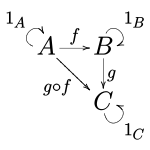
\includegraphics[scale=0.8]{150px-Category_SVG.png} 
\end{center}

\columnbreak
\pause

Beliebte Kategorien:\bigskip

\begin{itemize}
\pause\item Die Kategorie \textbf{Set}, von Mengen und Funktionen
\pause\item Die Kategorie \textbf{Cat}, von Kategorien und Funktoren
\pause\item Die Kategorie \textbf{Top}, von topologischen Räumen und stetigen Abbildungen
\end{itemize}

\end{multicols}

\end{frame}

%----------------------------------------------------------------------------------------
\subsection*{Zusammenfügen}

\begin{frame}

Fügen wir also zusammen, was wir gelernt haben:

\begin{itemize}
\pause\item Wir betrachten die Kategorie der Typen in \texttt{Haskell}: \texttt{Hask}.
\pause\item \texttt{Functor}s (die Typklasse) bilden \texttt{Hask} auf \texttt{Hask} ab, sind also Endofunktoren. 
\pause\item Nehmen wir einen dieser Endofunktoren als Basis eines Monoiden, brauchen wir noch ein neutrales Element und eine abgeschl. binäre Relation.
\pause\item $\eta : I \to M$ (unit) und $\mu : M \times M \to M$ (join) sind genau das.
\pause\item Ein \texttt{Functor} mit $\mu$ und $\eta$ ist eine Monade!
\end{itemize}

\pause\bigskip
\begin{center}
$\therefore$ \textit{\glqq Monaden sind Monoide in der Kategorie der Endofunktoren.\grqq}
\end{center}

\end{frame}

%----------------------------------------------------------------------------------------

\begin{frame}
\begin{center}

\includegraphics[scale=0.25]{thatsall.jpg} 
\end{center}
\end{frame}

\end{document}